%% This file was auto-generated by IPython.
%% Conversion from the original notebook file:
%% heat2.ipynb
%%
\documentclass[11pt,english,fleqn]{article}

%% This is the automatic preamble used by IPython.  Note that it does *not*
%% include a documentclass declaration, that is added at runtime to the overall
%% document.

\usepackage{amsmath}
\usepackage{amssymb}
\usepackage{graphicx}
\usepackage{ucs}
\usepackage[utf8x]{inputenc}

% needed for markdown enumerations to work
\usepackage{enumerate}

% Slightly bigger margins than the latex defaults
\usepackage{geometry}
\geometry{verbose,tmargin=3cm,bmargin=3cm,lmargin=2.5cm,rmargin=2.5cm}

% Define a few colors for use in code, links and cell shading
\usepackage{color}
\definecolor{orange}{cmyk}{0,0.4,0.8,0.2}
\definecolor{darkorange}{rgb}{.71,0.21,0.01}
\definecolor{darkgreen}{rgb}{.12,.54,.11}
\definecolor{myteal}{rgb}{.26, .44, .56}
\definecolor{gray}{gray}{0.45}
\definecolor{lightgray}{gray}{.95}
\definecolor{mediumgray}{gray}{.8}
\definecolor{inputbackground}{rgb}{.95, .95, .85}
\definecolor{outputbackground}{rgb}{.95, .95, .95}
\definecolor{traceback}{rgb}{1, .95, .95}

% Framed environments for code cells (inputs, outputs, errors, ...).  The
% various uses of \unskip (or not) at the end were fine-tuned by hand, so don't
% randomly change them unless you're sure of the effect it will have.
\usepackage{framed}

% remove extraneous vertical space in boxes
\setlength\fboxsep{0pt}

% codecell is the whole input+output set of blocks that a Code cell can
% generate.

% TODO: unfortunately, it seems that using a framed codecell environment breaks
% the ability of the frames inside of it to be broken across pages.  This
% causes at least the problem of having lots of empty space at the bottom of
% pages as new frames are moved to the next page, and if a single frame is too
% long to fit on a page, will completely stop latex from compiling the
% document.  So unless we figure out a solution to this, we'll have to instead
% leave the codecell env. as empty.  I'm keeping the original codecell
% definition here (a thin vertical bar) for reference, in case we find a
% solution to the page break issue.

%% \newenvironment{codecell}{%
%%     \def\FrameCommand{\color{mediumgray} \vrule width 1pt \hspace{5pt}}%
%%    \MakeFramed{\vspace{-0.5em}}}
%%  {\unskip\endMakeFramed}

% For now, make this a no-op...
\newenvironment{codecell}{}

 \newenvironment{codeinput}{%
   \def\FrameCommand{\colorbox{inputbackground}}%
   \MakeFramed{\advance\hsize-\width \FrameRestore}}
 {\unskip\endMakeFramed}

\newenvironment{codeoutput}{%
   \def\FrameCommand{\colorbox{outputbackground}}%
   \vspace{-1.4em}
   \MakeFramed{\advance\hsize-\width \FrameRestore}}
 {\unskip\medskip\endMakeFramed}

\newenvironment{traceback}{%
   \def\FrameCommand{\colorbox{traceback}}%
   \MakeFramed{\advance\hsize-\width \FrameRestore}}
 {\endMakeFramed}

% Use and configure listings package for nicely formatted code
\usepackage{listingsutf8}
\lstset{
  language=python,
  inputencoding=utf8x,
  extendedchars=\true,
  aboveskip=\smallskipamount,
  belowskip=\smallskipamount,
  xleftmargin=2mm,
  breaklines=true,
  basicstyle=\small \ttfamily,
  showstringspaces=false,
  keywordstyle=\color{blue}\bfseries,
  commentstyle=\color{myteal},
  stringstyle=\color{darkgreen},
  identifierstyle=\color{darkorange},
  columns=fullflexible,  % tighter character kerning, like verb
}

% The hyperref package gives us a pdf with properly built
% internal navigation ('pdf bookmarks' for the table of contents,
% internal cross-reference links, web links for URLs, etc.)
\usepackage{hyperref}
\hypersetup{
  breaklinks=true,  % so long urls are correctly broken across lines
  colorlinks=true,
  urlcolor=blue,
  linkcolor=darkorange,
  citecolor=darkgreen,
  }

% hardcode size of all verbatim environments to be a bit smaller
\makeatletter 
\g@addto@macro\@verbatim\small\topsep=0.5em\partopsep=0pt
\makeatother 

% Prevent overflowing lines due to urls and other hard-to-break entities.
\sloppy

\setlength{\mathindent}{0pt}
\setlength{\parindent}{0pt}
\setlength{\parskip}{8pt}
\begin{document}

Isi Denklemi
\[ \frac{\partial u}{\partial t} = \frac{\partial^2u}{\partial x^2} \]
olarak gosterilen denklem fizikte isi denklemi olarak bilinir, u
fonksiyonu iki degiskenlidir $u(x,t)$. Ornek icin bu denklemin cozumunu
tek boyutta gosterecegiz, yani bir genisligi onemli olmayan bir demir
cubugu uzerinde isinin dagilmasi konusuna bakacagiz, boyutu temsil icin
$x$ degiskeni kullanilacak. $t$ degiskeni zamani temsil ediyor olacak.
Baslangic sartlari (initial conditions) olarak isinin t=0 aninda demir
cubuk uzerinde $x$'e bagli bir sinus fonksiyonu ile dagildigini
farzedecegiz, sinir sartlari ise (boundary conditions) cubugun iki
ucunun sifir derecede tutulmasi olacak. Sonucta isinin nereye gidecegini
tahmin ederek te soyleyebiliriz -- isi demirin iki ucundan kacarak tum
cubuk boyunca sifir dereceye inecektir.

Ustteki denklem bir kismi diferansiyel denklemdir (partial differential
equation).

Matematiksel cozumler ya analitik, ya da yaklasiksal olur. Biz bu ornegi
cozmek icin yaklasiksal, hesapsal bir teknik kullanacagiz. Elimizde bir
diferansiyel denklem varsa cozum bulmak demek bir fonksiyon bulmak
demektir, bir sayi degil; yaklasiksal yontemle de oyle bir $u$
fonksiyonu bulacagiz ki, test / belli noktalarda gercek fonksiyonla
olabildigince ayni sonuclar verecek.

Cozumde sinirli farklar (finite differences) denen bir metot
kullanilacak. Bu yaklasiksal metotta calculus'un sonsuz ufakliklar icin
kullanilan turevleri, bildigimiz sayisal cikartma islemi uzerinden
tanimlanan ``farkliliklara'' donusecekler. Mesela $d^2/dx^2$ nedir?
$x$'e gore turevin turevidir, hesapsal olarak ise farkin farkidir.
Sonsuzluktan yaklasiga soyle geceriz: Eger $u_{j,i}$ bir 2 boyutlu dizin
uzerinde $u$ fonksiyonunun sayisal degerlerini tasiyor olsaydi, ve
$j, i$ indis degerleri $t, x$'i temsil ediyorlar ise, $x$ uzerinden
birinci turev yani birinci fark (first difference) soyle olur:
\[ \frac{u_{j,i+1}-u_{j,i}}{h} \]
$h$ hangi degiskenin farkini aliyorsak, o farkin buyuklugunu tanimlayan
aralik degeridir, $h=\Delta x$, ve $u_{j,i+1} = u(t,x + \Delta x)$.

Ikinci fark, farkin farkidir:
\[ \frac{1}{h}
\bigg[
\bigg( \frac{u_{j,i+1}-u_{j,i}}{h} \bigg) -
\bigg( \frac{u_{j,i}-u_{j,i-1}}{h} \bigg)
\bigg] 
 \]
\begin{equation} = \frac{u_{j,i+1}-2u_{j,i}+u_{j,i-1}}{h^2} \label{diff} \end{equation}

Bu carpimi tum $i$ degerleri icin ve matris uzerinden temsil etmenin
yolu sudur: Bir ikinci farkliliklar matrisi A yaratiriz:
\[ 
A = \frac{1}{\Delta x^2}
\left[ \begin{array}{ccccccc}
-2 & 1 & 0 & 0 \ldots 0 & 0 & 0 \\
1 & -2 & 1 & 0 \ldots 0 & 0 & 0 \\
\vdots & \vdots & \vdots & \vdots & \vdots & \vdots \\
0 & 0 & 0 & 0 \ldots 1 & -2 & 1 \\
0 & 0 & 0 & 0 \ldots 0 & 1 & -2
\end{array} \right]
 \]
Ve u degerlerinin bir vektor icine cekeriz:
\[ U_j =
\left[ \begin{array}{c}
u_{j,0} \\
u_{j,1} \\
u_{j,2} \\
\vdots \\
u_{j,n}
\end{array} \right]
 \]
$AU_j$ carpiminin \ref{diff} denklemindeki toplamlari her u icin teker
teker verecegini gorebiliriz. Indislerden $j$ zaman, $i$ mesafedir, yani
ustteki denklem simdilik sadece mesafeyi yani $x$'i parcalara bolmustur.

Zamani da modele dahil edelim ve cozumu elde etmeye ugrasalim. Isi
denkleminin tamamini simdiye kadar elde ettiklerimizi kullanarak ve
ayriksal olarak yazalim:

\begin{equation}
\frac{U_{j+1}-U_j}{\Delta t} = AU_j \label{main}
\end{equation}

$\frac{\partial^2u}{\partial x^2} \approx AU_j$, ve
$\frac{\partial u}{\partial t} \approx (U_{j+1}-U_j) / \Delta t$ olarak
alindi. $U_j$ tanimindaki $j$ indisi zaman icin kullaniliyor, mesafe
yani $x$'i temsil eden indislerin tamami $U$'nun icinde var zaten.

Yaklasiksal tekniklerden Crank-Nicholson'a gore $AU_j$'i ardi ardina iki
zaman indisi uzerinden hesaplanan bir ortalama olarak temsil edebiliriz,
yani
\[ AU_j \approx \frac{1}{2}(AU_{j+1}+AU_j) \]
Niye bu acilim yapildi? Cunku elimizde $U_{j+1}$ ve $U_j$ degerleri var,
bu degerleri tekrar ortaya cikararak bir ``denklem sistemi'' yaratmis
olacagiz, iki bilinmeyen icin iki formul yanyana gelebilecek ve cozume
erisilebilecek.

Ustteki formulu \ref{main} denklemindeki $AU_j$ degerleri icinkullanalim
ve tekrar duzenleyelim.
\[ \frac{\Delta t}{2}AU_{j+1} + \frac{\Delta t}{2}AU_j = U_{i+1} - U_i  \]\[ U_{i+1} - \frac{\Delta t}{2}AU_{j+1} = U_i + \frac{\Delta t}{2}AU_j  \]\[ (I - \frac{\Delta t}{2}A) U_{j+1} = (I + \frac{\Delta t}{2}A)U_i \]
Artik bu formulu lineer cebirden bilinen $Ax=b$ formuna sokarak
cozebiliriz. Forma gore formulun sag tarafi $b$ olur, sol tarafta
parantez ici A olacak, $U_{j+1}$ ise bilinmeyen $x$ olacak (bizim
$x$'ten farkli). Hesapsal kodlar bir dongu icinde, her zaman dilimi icin
bilinmeyen $U_{j+1}$ degerini bulacak. Dongunun sonunda yeni $U_{j+1}$
eski $U_j$ olacak ve hesap devam edecek.

Sinir Sartlari

Her iki ucta $u$'nun sifir olma sarti uygulamali matematikte Dirichlet
sinir sarti olarak biliniyor. Bu sart $A$ matrisinin olusturulmasi
sirasinda kendiliginden olusuyor. Ufaltilmis bir D2 matrisi uzerinde
gostermek gerekirse,
\[ \left[ \begin{array}{ccccc}
1 & -2 & 1 & 0 & 0 \\
0 & 1 & -2 & 1 & 0 \\
0 & 0 & 1 & -2 & 1
\end{array} \right]
 \]
degerlerinin her satirinin \ref{diff} denklemini temsil ettigini
soylemistik. Eger sartlarimizdan biri $u_1$ ve $u_5$'un sifir olmasi
ise, carpim sirasinda ona tekabul eden D2'nin en soldaki ve en sagdaki
kolonlarin tamamen sifir yapmamiz yeterli olurdu, cunku carpim sirasinda
$U_j$ icinde o kolonlar $u_1$ ve $u_5$ ile carpilip onu sifir
yaparlardi. O zaman yeni matris soyle olurdu:
\[ 
\left[ \begin{array}{ccccc}
0 & -2 & 1 & 0 & 0 \\
0 & 1 & -2 & 1 & 0 \\
0 & 0 & 1 & -2 & 0
\end{array} \right]
 \]
Bu isler. Alternatif olarak sifir kolon yerine, o kolonlari tamamen
matristen atabilirdik, ayni sekilde $u$ degerlerini uretirken birinci ve
sonuncu degerleri de atmamiz gerekirdi, nasil olsa onlar ``bilinmeyen''
degisken degiller. Bu yeni matris soyle olurdu:
\[ \left[ \begin{array}{ccc}
-2 & 1 & 0  \\
1 & -2 & 1  \\
0 & 1 & -2 
\end{array} \right]
\]
Alttaki kod icinde x = x{[}1:-1{]} ibaresi $x$ ve dolayli olarak $u$'nun
ilk ve son degerlerini atmak icin kullanilmakta.

Seyrek (sparse) matrisler kullanarak cozum altta.

\begin{codecell}
\begin{codeinput}
\begin{lstlisting}
"""
	This program solves the heat equation
		u_t = u_xx
	with dirichlet boundary condition
		u(0,t) = u(1,t) = 0
	with the Initial Conditions
		u(x,0) = 10*sin( pi*x )
	over the domain x = [0, 1]
 
	The program solves the heat equation using a finite difference
	method where we use a center difference method in space and
	Crank-Nicolson in time.
"""
 
import scipy as sc
import scipy.sparse as sparse
import scipy.sparse.linalg
import time
from IPython.display import clear_output
f, ax = plt.subplots()

 
# Number of internal points
N = 200
 
# Calculate Spatial Step-Size
h = 1/(N+1.0)
 
# Create Temporal Step-Size, TFinal, Number of Time-Steps
k = h/2
TFinal = 1
NumOfTimeSteps = 120
 
# Create grid-points on x axis
x = np.linspace(0,1,N+2)
x = x[1:-1]

# Initial Conditions
u = np.transpose(np.mat(10*np.sin(np.pi*x)))
 
# Second-Derivative Matrix
data = np.ones((3, N))
data[1] = -2*data[1]
diags = [-1,0,1]
D2 = sparse.spdiags(data,diags,N,N)/(h**2)

# Identity Matrix
I = sparse.identity(N)
 
# Data for each time-step
data = []
 
for i in range(NumOfTimeSteps):
	# Solve the System: 
	#
	# (I - k/2*D2) u_new = (I + k/2*D2)*u_old
	#
	A = (I -k/2*D2)
	b = ( I + k/2*D2 )*u
	u = np.transpose(np.mat(sparse.linalg.spsolve(A, b)))
        ax.plot(x, u)
    	ax.axis((0,1,0,10.1))
    	clear_output()
    	display(f)
	ax.cla()
\end{lstlisting}
\end{codeinput}
\begin{codeoutput}
\begin{center}
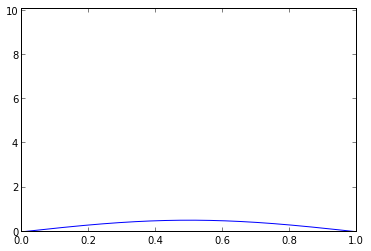
\includegraphics[width=0.7\textwidth]{heat2_files/heat2_fig_00.png}
\par
\end{center}
\begin{center}
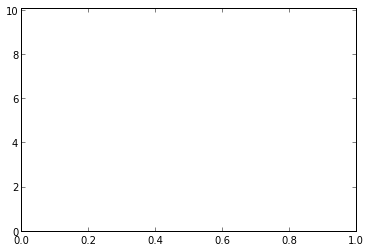
\includegraphics[width=0.7\textwidth]{heat2_files/heat2_fig_01.png}
\par
\end{center}
\end{codeoutput}
\end{codecell}
Seyrek matrislerden olmadan, normal matris kullanarak olan cozum altta.

\begin{codecell}
\begin{codeinput}
\begin{lstlisting}
import scipy.linalg
from IPython.display import clear_output
f, ax = plt.subplots()

# Number of internal points
N = 200

# Calculate Spatial Step-Size
h = 1/(N+1.0)
k = h/2

x = np.linspace(0,1,N+2)
x = x[1:-1] # get rid of the '0' and '1' at each end

# Initial Conditions
u = np.transpose(np.mat(10*np.sin(np.pi*x)))

# second derivative matrix
I2 = -2*np.eye(N)
E = np.diag(np.ones((N-1)), k=1)
D2 = (I2 + E + E.T)/(h**2)

I = np.eye(N)

TFinal = 1
NumOfTimeSteps = 100

for i in range(NumOfTimeSteps):
    # Solve the System: 
    # (I - k/2*D2) u_new = (I + k/2*D2)*u_old
    A = (I - k/2*D2)
    b = np.dot((I + k/2*D2), u)
    u = scipy.linalg.solve(A, b)
    ax.plot(x, u)
    ax.axis((0,1,0,10.1))
    clear_output()
    display(f)
    ax.cla()    

\end{lstlisting}
\end{codeinput}
\begin{codeoutput}
\begin{center}
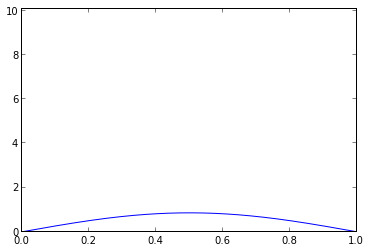
\includegraphics[width=0.7\textwidth]{heat2_files/heat2_fig_02.png}
\par
\end{center}
\begin{center}
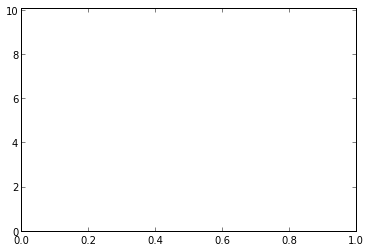
\includegraphics[width=0.7\textwidth]{heat2_files/heat2_fig_03.png}
\par
\end{center}
\end{codeoutput}
\end{codecell}

\end{document}
